\part{Entrega 1}


\section{Introducción}
Las estructuras que se utilizan en el espacio deben contar con una serie de características que les permitan operar y cumplir con su función de forma eficiente y segura. Una de estas características es la relación de masa estructural y la longitud de la estructura con las frecuencias y modos de vibración de la misma. Si estos requisitos no se cumplen, mandar la estructura al espacio además de ser costoso, puede ser peligroso para la tripulación y la misión.

En este informe se estudiarán varias relaciones de masa estructural para obtener un área óptima de un reticulado, junto con la determinación de los modos de vibración que sean mayores a 0.1 Hz, ya que esta es una frecuencia que se considera segura en el espacio.

Para cumplir con este objetivo, se emplearán la librería OpenSeesPy para el análisis estructural y la identificación de las frecuencias y modos de vibración de la estructura, y PyVista para la visualización de los datos obtenidos.
\newpage
\section{Modelo}
Lo primero que se hizo para poder modelar de forma precisa, fue la creación de una función la cual permitiera la creación de un reticulado con las dimensiones y cantidad de vanos que el usuario deseara, que es el lo que se muestra a continuación:

\begin{lstlisting}
def conectar_nodos_cuadrado(node_tags, element_id, A, material_id, gamma, elements):
    for i in range(len(node_tags)):
        j = (i + 1) % len(node_tags)  # Cerrar el ciclo conectando el último con el primero
        #print(f'{i=}, {j=}')
        elements.append(crear_elemento_truss(element_id, node_tags[i], node_tags[j], A, material_id, gamma))
        element_id += 1

    #Ahora conecto una diagonal
    if node_tags[0] == 1:
        #Estoy en el primer elemento
        elements.append(crear_elemento_truss(element_id, node_tags[i], node_tags[j]+1, A, material_id, gamma))
        element_id += 1

    elif node_tags[-1] == num_capas*4 + 4:
        #Estoy en el ultimo elemento
        elements.append(crear_elemento_truss(element_id, node_tags[i], node_tags[j]+1, A, material_id, gamma))
        element_id += 1

    else:
        #Agrego dos diagonales
        elements.append(crear_elemento_truss(element_id, node_tags[i], node_tags[j]+1, A, material_id, gamma))
        element_id += 1

        elements.append(crear_elemento_truss(element_id, node_tags[i]-1, node_tags[j], A, material_id, gamma))
        element_id += 1
    return element_id
\end{lstlisting}

Así, los reticulados para 2, 4, 8 y 16 módulos se visualizan de la siguiente forma.

\begin{figure}[H]
    \begin{minipage}[b]{0.5\textwidth}
        \centering
        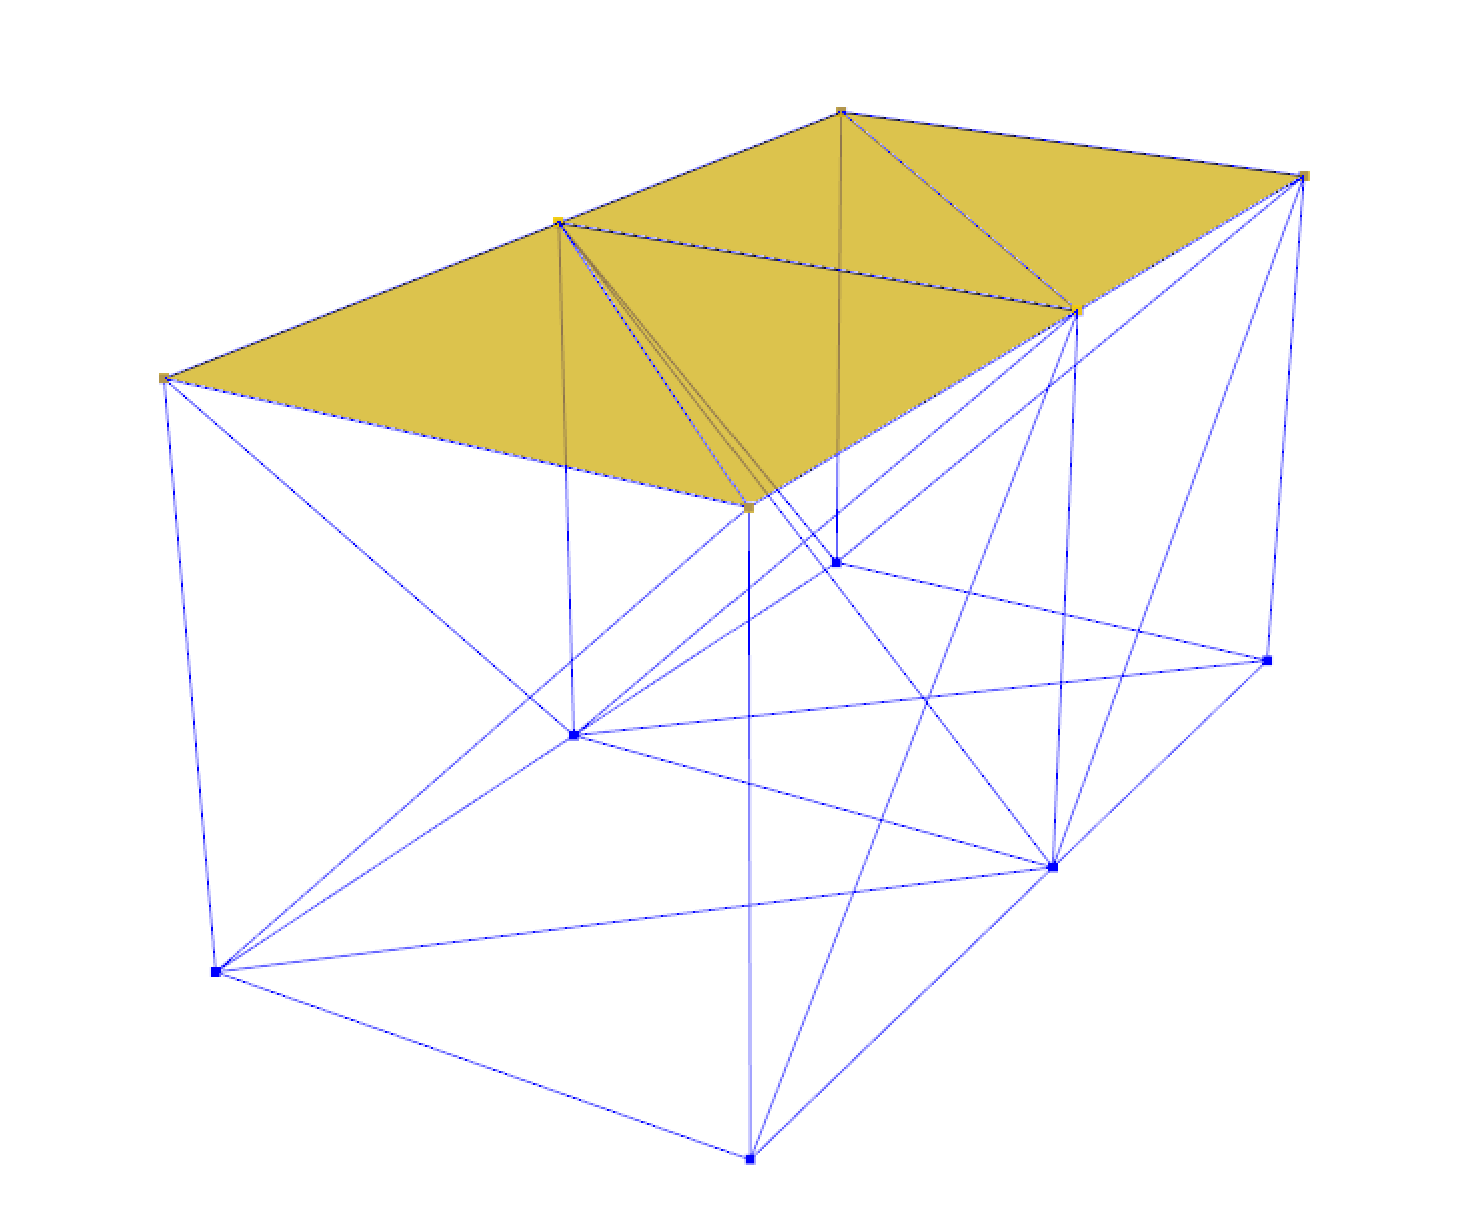
\includegraphics[width=\textwidth]{FOTOS/2.png}
        \caption{Reticulado de 2 módulos.}
    \end{minipage}
    \hfill
    \begin{minipage}[b]{0.5\textwidth}
        \centering
        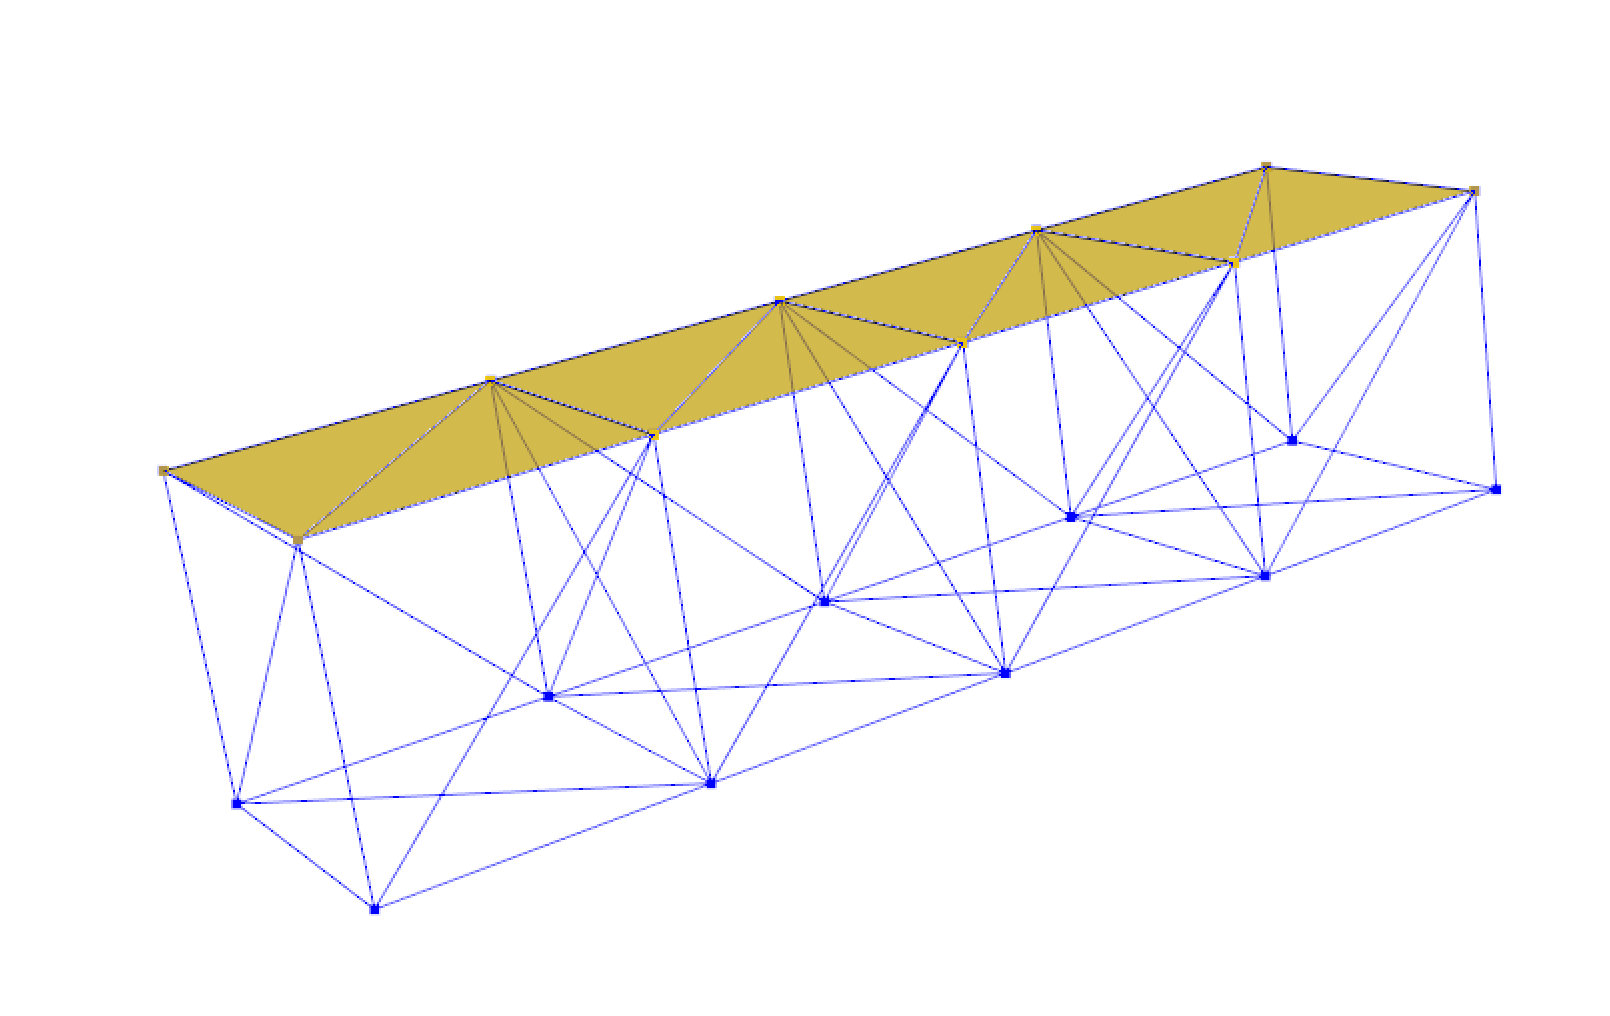
\includegraphics[width=\textwidth]{FOTOS/4.png}
        \caption{Reticulado de 4 módulos.}
    \end{minipage}
\end{figure}

\begin{figure}[H]
    \begin{minipage}[b]{0.5\textwidth}
        \centering
        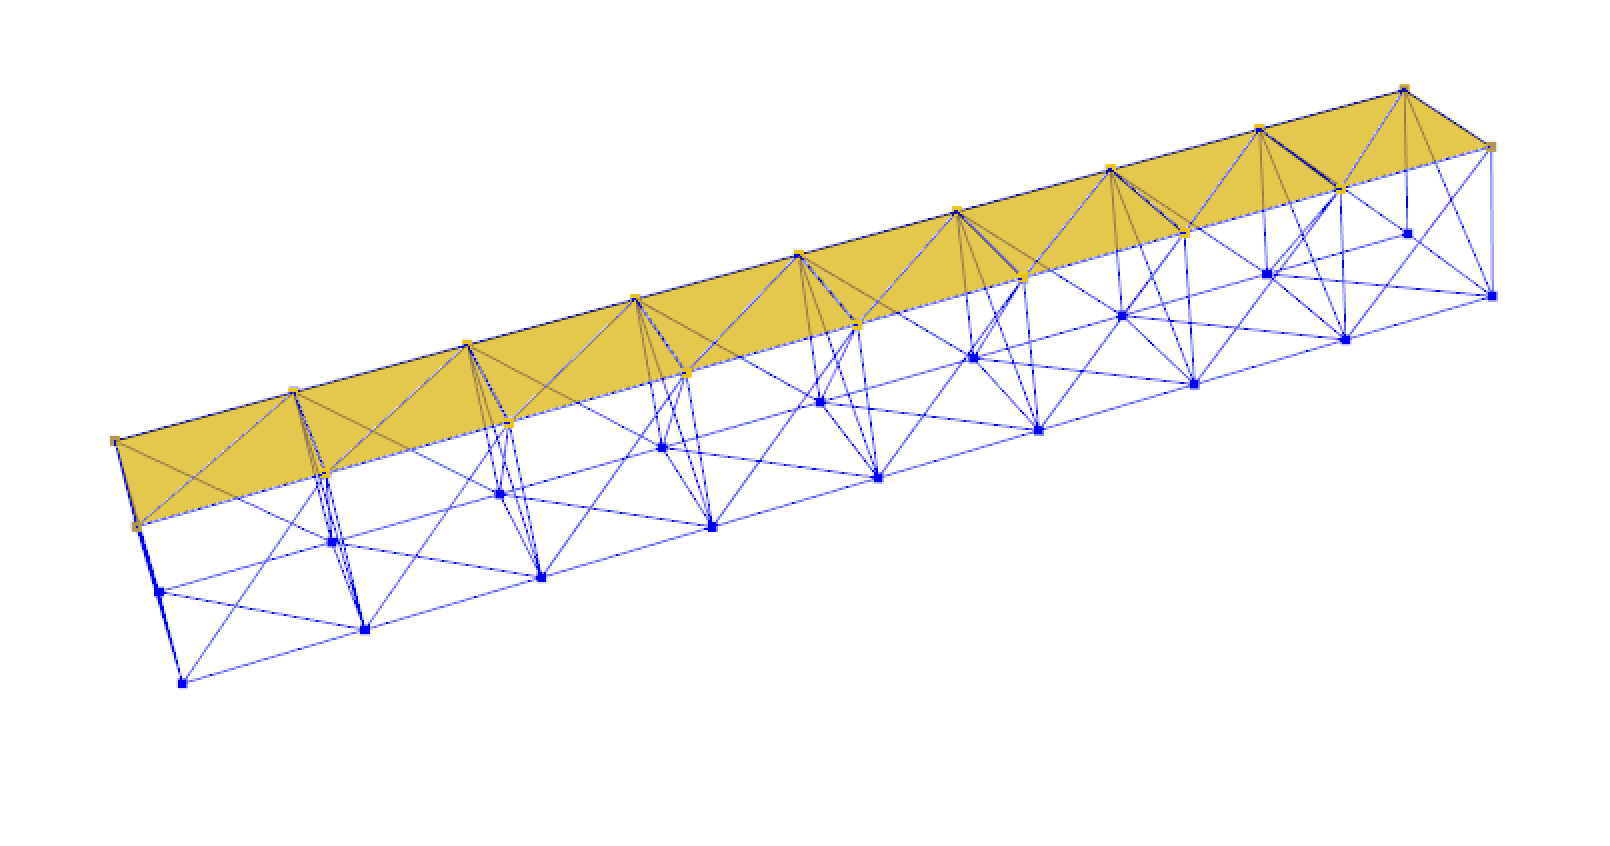
\includegraphics[width=\textwidth]{FOTOS/8.png}
        \caption{Reticulado de 8 módulos.}
    \end{minipage}
    \hfill
    \begin{minipage}[b]{0.5\textwidth}
        \centering
        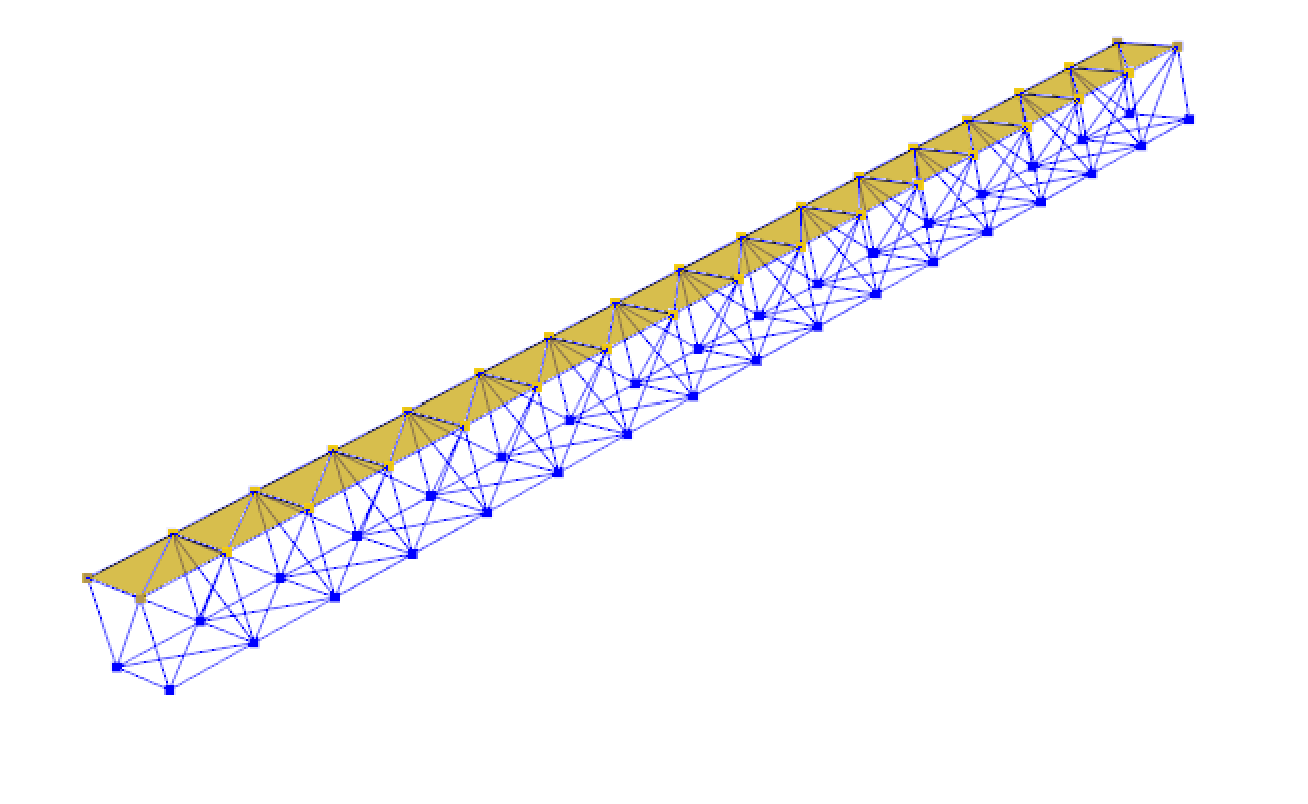
\includegraphics[width=\textwidth]{FOTOS/16.png}
        \caption{Reticulado de 16 módulos.}
    \end{minipage}
\end{figure}

Luego, se procedió a la obtención de las frecuencias y modos de vibración de la estructura, para lo cual se utilizó el comando \texttt{eigen} de OpenSeesPy. Con los datos obtenidos, se procedió a la visualización de los modos de vibración de la estructura, para lo cual se utilizó PyVista. A continuación, se muestran las estructuras con su deformación en el modo 1 de vibración, como ejemplo.

\begin{figure}[H]
    \begin{minipage}[b]{0.5\textwidth}
        \centering
        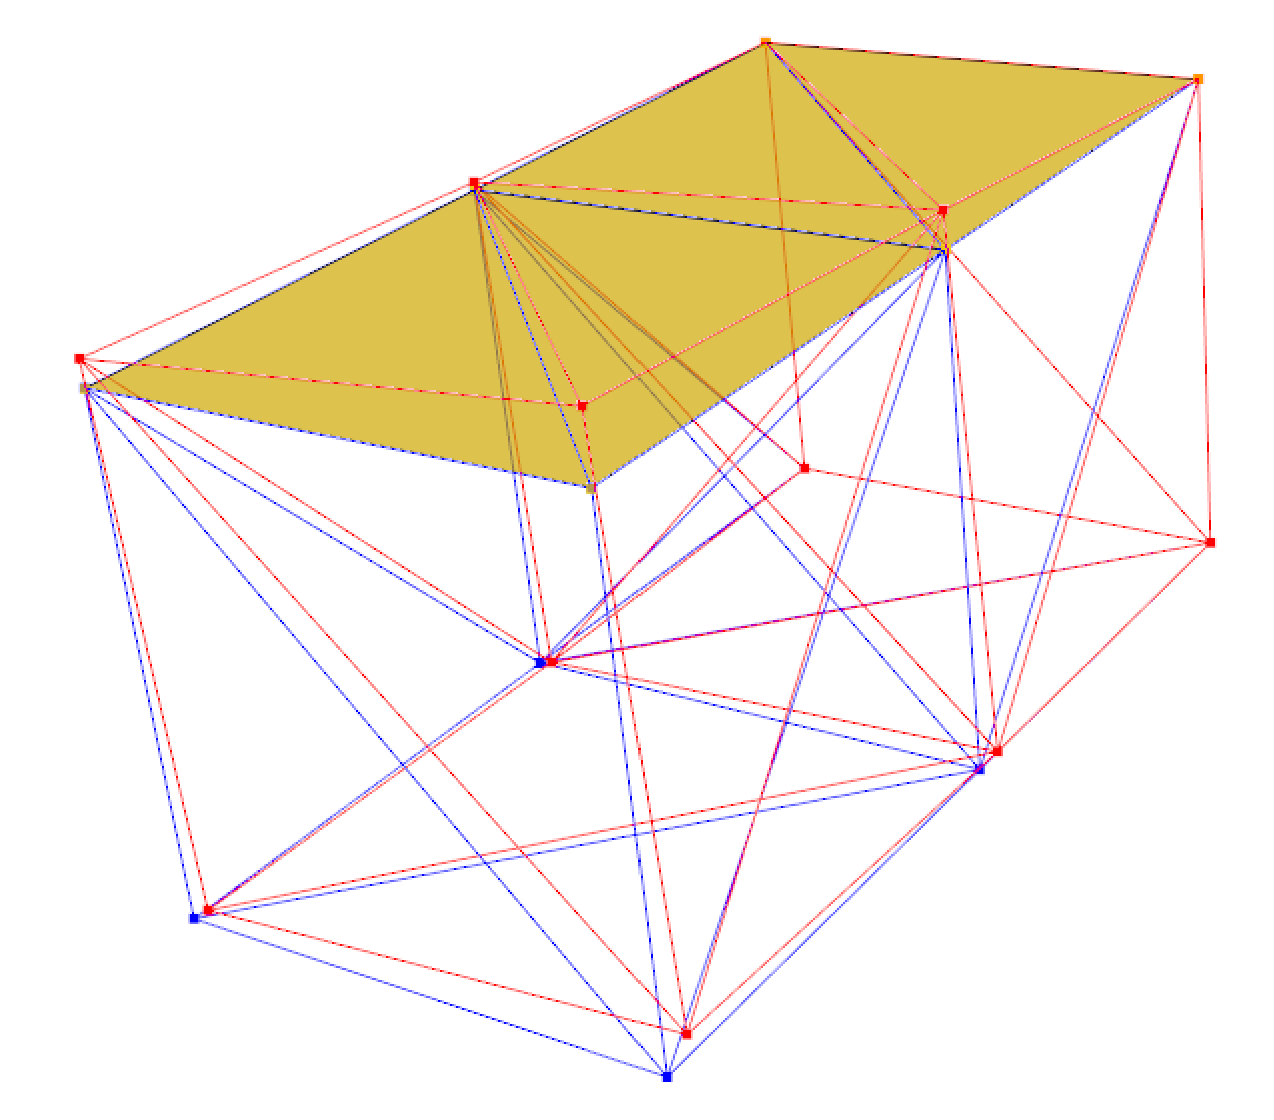
\includegraphics[width=\textwidth]{FOTOS/m1_2.png}
        \caption{Reticulado de 2 y su modo 1.}
    \end{minipage}
    \hfill
    \begin{minipage}[b]{0.5\textwidth}
        \centering
        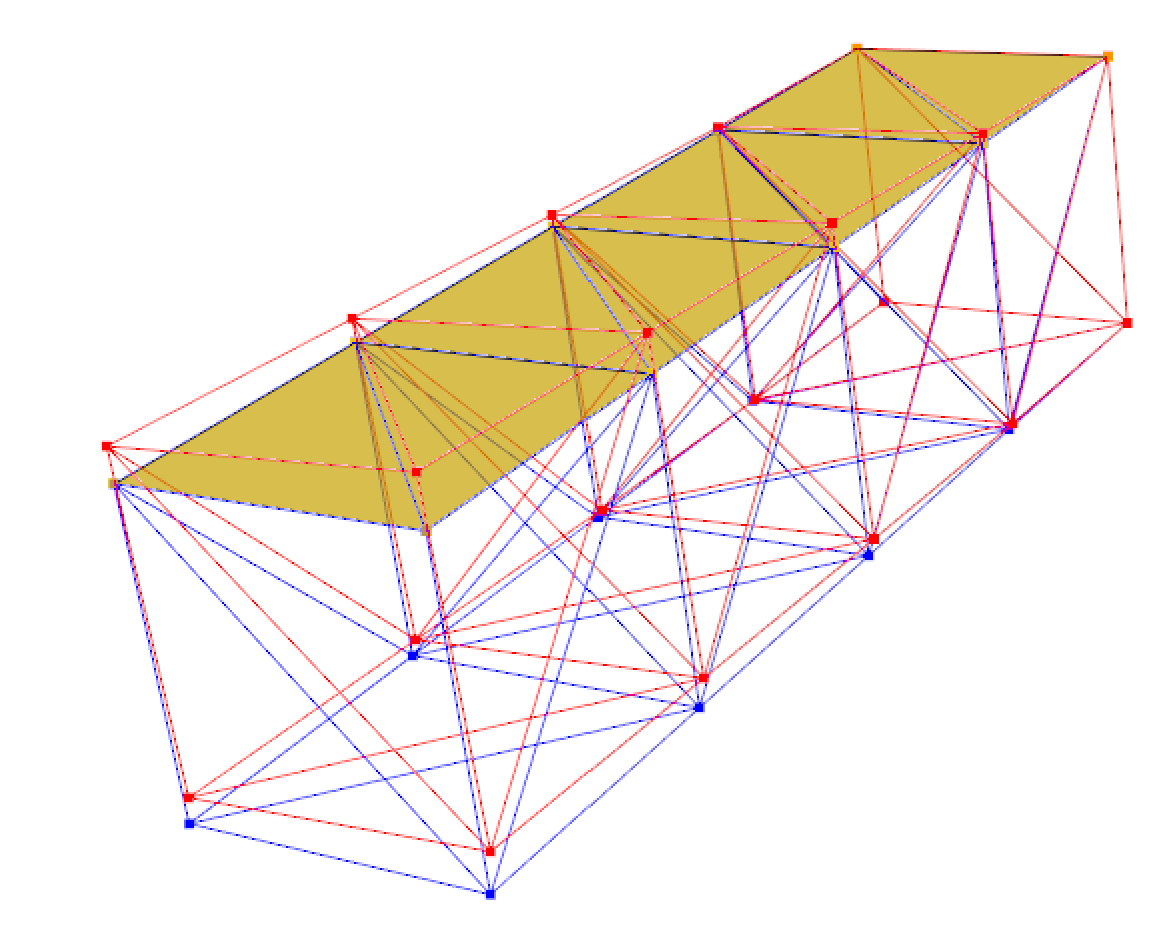
\includegraphics[width=\textwidth]{FOTOS/m1_4.png}
        \caption{Reticulado de 4 y su modo 1.}
    \end{minipage}
\end{figure}

\begin{figure}[H]
    \begin{minipage}[b]{0.5\textwidth}
        \centering
        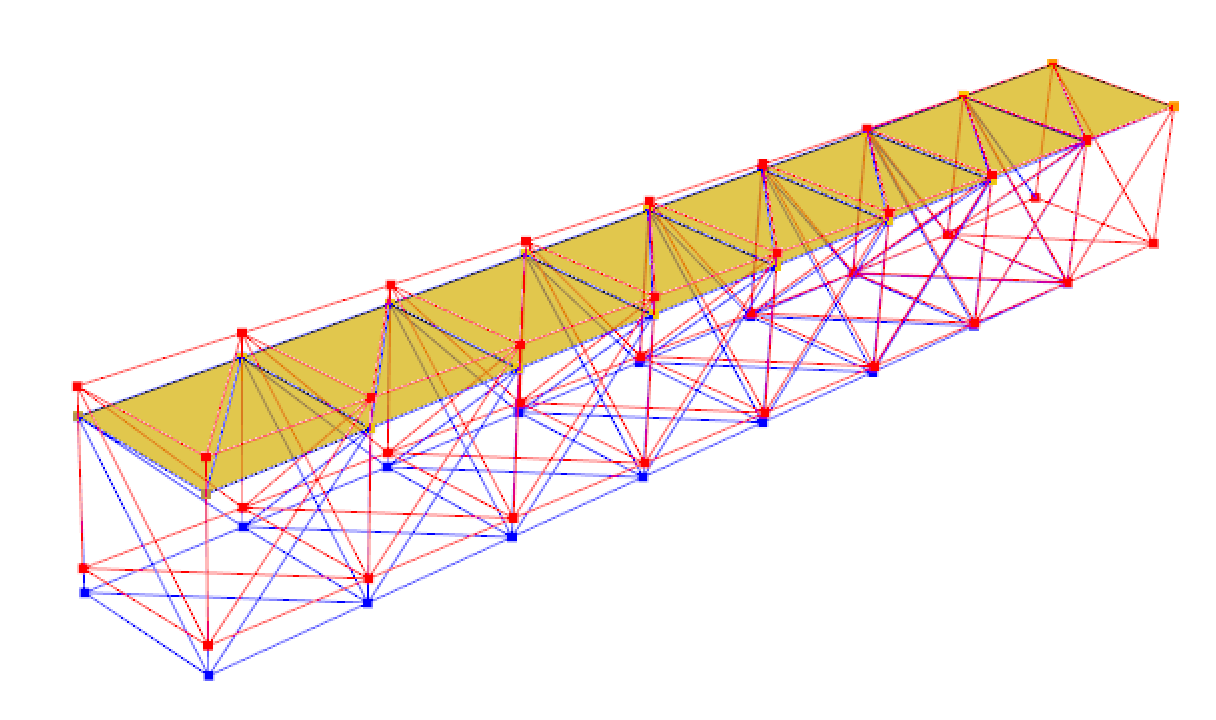
\includegraphics[width=\textwidth]{FOTOS/m1_8.png}
        \caption{Reticulado de 8 y su modo 1.}
    \end{minipage}
    \hfill
    \begin{minipage}[b]{0.5\textwidth}
        \centering
        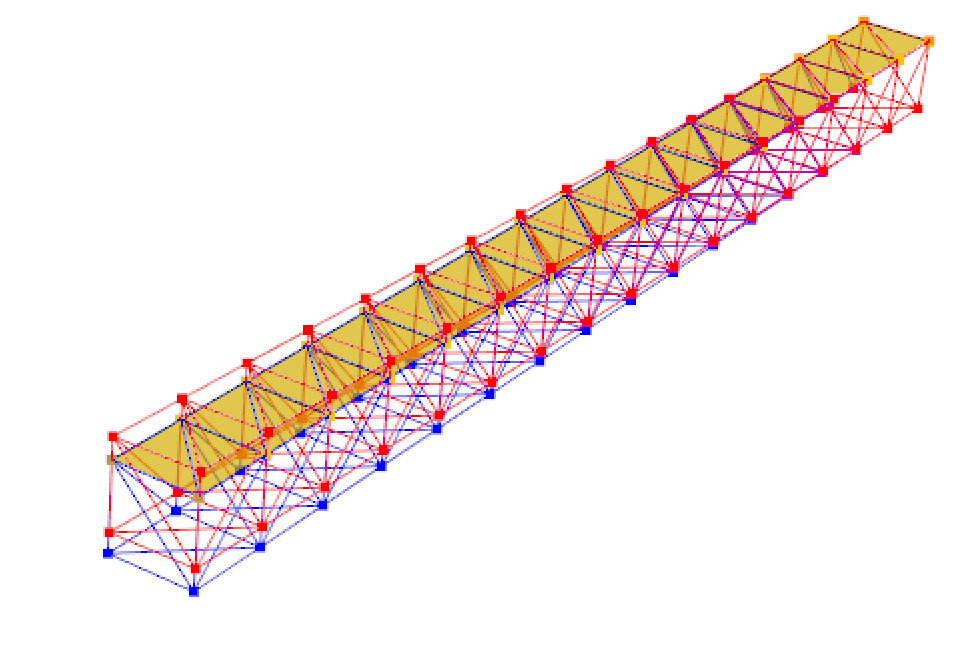
\includegraphics[width=\textwidth]{FOTOS/m1_16.png}
        \caption{Reticulado de 16 y su modo 1.}
    \end{minipage}
\end{figure}

Posteriormente, se procedió a calcular la relación de masa estructural con respecto a los paneles solares, para lo cual se utilizó la siguiente fórmula:

\begin{equation}
    \text{RME} = \frac{\text{Masa de la estructura}}{\text{Masa de los paneles solares}} \cdot 100
\end{equation}

Finalmente, se fueron calibrando los diámetros internos y externos de los tubos de la estructura, para obtener una relación de masa estructural que cumpliera con los siguientes porcentajes: 10\%, 20\%, 30\%


\section{Resultados}

\subsection{Análisis}



\section{Conclusiones}